
\subsection{The Binomial Distribution}

\ssn{An important example} 
What is the probability that on rolling three D6 I get exactly one `6'? 

There are exactly three routes through the tree that give this outcome and each has probability 
 \[
      \left( \frac16 \right) \left( \frac56 \right)^2 = \frac{25}{216}.
 \]
Thus the probability is 
 \[
     3 \frac{25}{216} = \frac{25}{72}. 
 \] 
\end{n}

\ssn{A generalisation}
Let us consider a general version of the problem.  Supposing we have a process that each time it is carried out produces independently a ``success'' (S) with probability $p$ or a failure (F) with probability $q=1-p$. In the examples in \S\ref{mp2}, success is finding a faulty component or correctly guessing the answer to a question.  We are assuming that each execution of the process is ``independent'', meaning that its success or failure  each time is not influenced by what might have happened before.  If we now repeat this process $n$ times, what is the probability that we get exactly $k$ successes? 
\end{n}




\ssn{Example} 
Suppose $n=10$ and $k=7$ and $p=1/4$. One particular sequence of successes and failures is $SSFFSSFSSS$. Thinking of a large probability tree, the probability of this exact sequence is 
 \[
    ppqqppqppp = p^k q^{n-k} = p^7 q^3 = \left( \frac14 \right)^7 \, \left( \frac34 \right)^3   = \frac{3^3}{4^{10}}
\]
This probability is the same for all the different sequences with seven successes. 

How many other sequences  are there with precisely seven S's?  That is the same question as asking how many ways are there of choosing seven things from ten.  It is the Binomial coefficient
 \[
       \binom{10}7 = \frac{10!}{7! \,3!} = 120. 
  \]
Adding all these possibilities, the probability of three successes in eight trials is exactly 
  \[
     \binom{10}7 p^k q^{n-k} = 120 \frac{3^3}{4^{10}} \approx 0.0031. 
  \]
\end{n}

\sse{}
Note that we have just derived the probability of getting exactly 7 out of 10 by guessing in our multiple choice quiz. Work out the probability of getting 8, 9 and 10 out of 10 and hence answer our second motivating problem. 
\end{e}

\sss
\[
    \binom{10}{7} \left( \frac13\right)^7 \left( \frac23 \right)^3 +  
    \binom{10}{8} \left( \frac13\right)^8 \left( \frac23 \right)^2 +  
    \binom{10}{9} \left( \frac13\right)^9 \left( \frac23 \right)^1 +  
    \binom{10}{10} \left( \frac13\right)^{10} \left( \frac23 \right)^0  \approx 0.019661636.
 \]
 (I give many decimal places because leaving out the 1/10 possibility only affects the fifth decimal place!) 
\end{s}


\ssn{} 
For the general problem, the probability of $k$ successes in $n$ trials is as follows.  
\tcb 
\ul{Binomial distribution} 
  \[
       \PP( \text{$k$ successes}) =  \binom nk p^k q^{n-k} =  \frac{n!}{k! \, (n-k)!} p^k q^{n-k}. 
  \]
 \etcb 
\end{n}

\ssn{Example}
I roll a D6 twelve times.  How likely is it that I roll precisely two sixes?   Here, $n=12, k=2$ and $p=1/6$. So the answer is 
 \[
    \binom{12}2 \left(\frac{1}{6}\right)^2  \left(\frac{5}{6}\right)^{10}
     \approx 0.296.
 \]
\end{n}

\sse{Exercise}
I toss a fair coin 6 times.  How likely is it that I roll $k$ heads where $k=0,1,2,3,4,5,6$? 
\end{e}
\sss 
Use the formula with $n=6$ and $p=1/2$.  For instance, $\PP(k=3) = 20/64 = 5/16$. 
\end{s}



\begin{table}[h]  
  \begin{tabular}{cc} 
    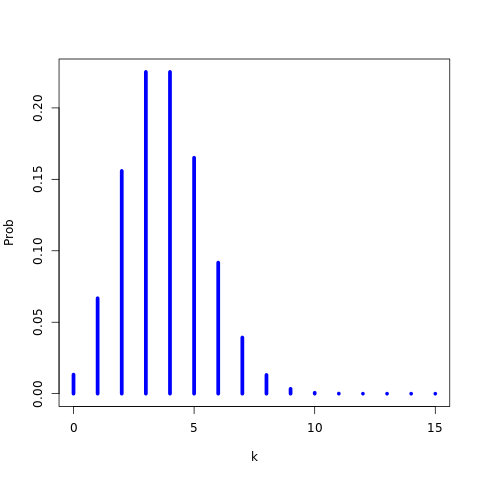
\includegraphics[width=0.45\textwidth]{images/binom15P25.png} & 
    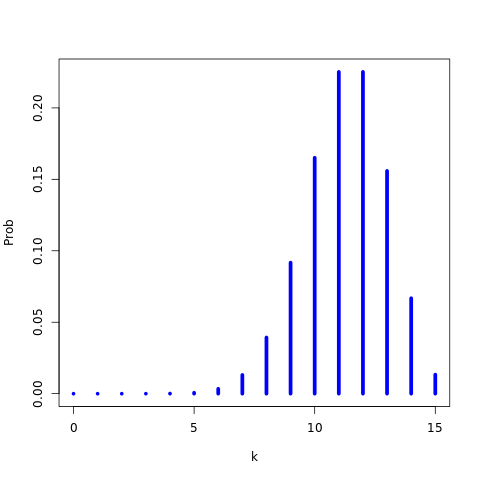
\includegraphics[width=0.45\textwidth]{images/binom15P75.png} \\
     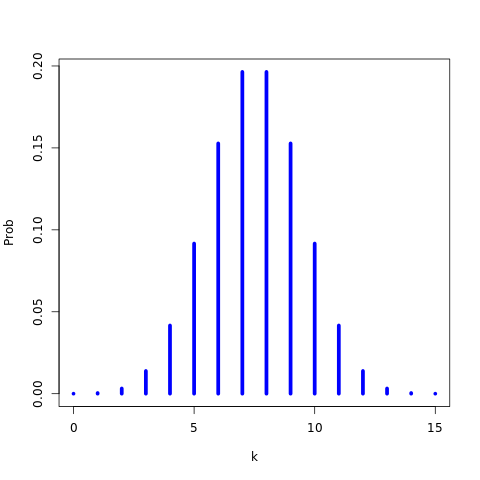
\includegraphics[width=0.45\textwidth]{images/binom15P5.png} & 
    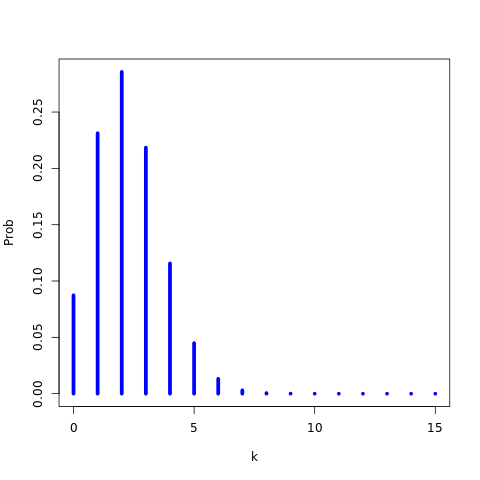
\includegraphics[width=0.45\textwidth]{images/binom15P15.png} \\
  \end{tabular}
 \caption{\label{binpics} Binomial with $n=15$ and $p=0.15, 0.25, 0.5, 0.75$ in some order}
\end{table}


\sse
In table~\ref{binpics} ``probability mass functions'' for Binomial distributions with different probabilities are plotted. The height of each vertical bar is the probability of the corresponding outcome. Which is which?
\end{e}

\sss
The top row has $p=0.25$ and $p=0.75$. Note the symmetry between them. 
The bottom two are $p=0.5$ (note the symmetry about its centre) and $p=0.15$. 
\end{s}

\sse{}
\begin{enumerate}
    \item 
Compute the `Red v Blue' and `Green v Red' probabilities with a tree.
 \item Compute the win probability of Blue versus Green where the game is to roll two blue dice versus two green dice with the higher total winning. 
\end{enumerate}
Answers to these can be found in the Workshop 1 solutions. 
\end{e}

